\usetikzlibrary{shapes}%add to preambule if the main file does not compile

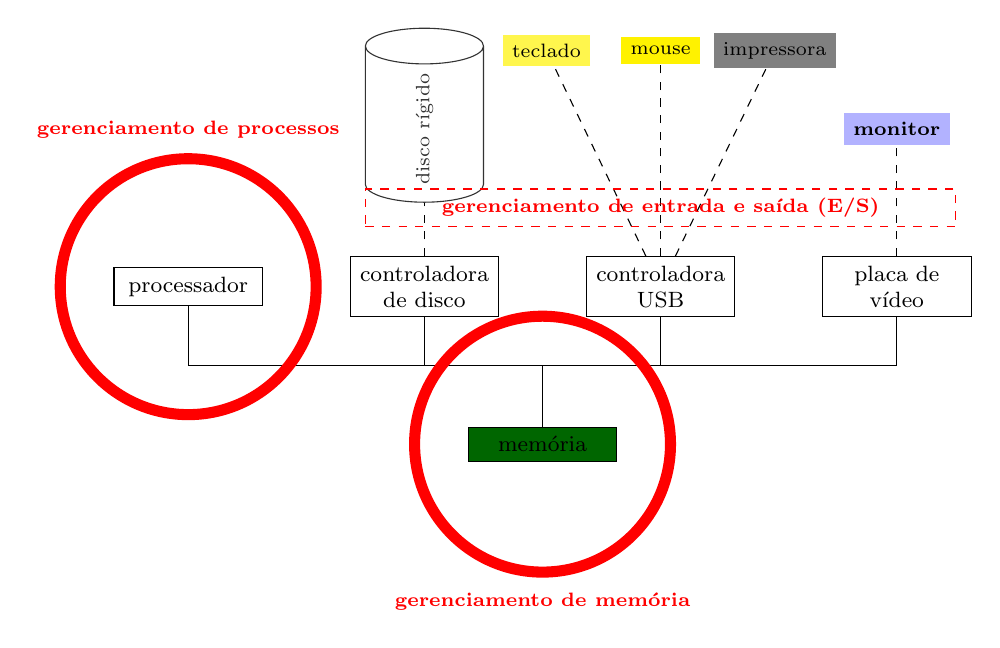
\begin{tikzpicture}[control/.style={text width=1.65cm,align=center,font=\footnotesize,draw},
    every path/.style={draw},device/.style={fill=yellow,font=\scriptsize,minimum width=1cm},
    device connection/.style={dashed},
    disk/.style={black!80,font=\scriptsize,cylinder,minimum width=1.5cm,rotate=90,draw},
    os module/.style={minimum size=3.25cm,circle,red,line width=4,text width=2cm,draw},
    module label/.style={red,font=\bf\scriptsize}]

    \def\dx{3cm}
    \def\dy{2cm}
    
    \node[control] (proc) at (0,0) {processador};
    \node[control] (disk controller) at (\dx,0) {controladora de disco};
    \node[control] (usb controller) at (2*\dx,0) {controladora USB};
    \node[control] (video card) at (3*\dx,0) {placa de vídeo};
    \node[control,fill=green!40!black] (mem) at (1.5*\dx,-\dy) {memória};

    \path (proc) -- +(0,-0.5*\dy) -- +(3*\dx,-0.5*\dy) -- +(video card);
    \path (\dx,-0.5*\dy) -- +(disk controller);
    \path (2*\dx,-0.5*\dy) -- +(usb controller);
    \path (1.5*\dx,-0.5*\dy) -- +(mem);

    \node[disk] (hd) at (\dx,\dy) {disco rígido};
    \path[device connection] (disk controller) -- (hd);

    \node[device] (mouse) [above of=usb controller,yshift=\dy] {mouse};
    \node[device,fill=gray] (printer) [right of=mouse,xshift=.15*\dx] {impressora};
    \node[device,fill=yellow!70] (keyboard) [left of=mouse,xshift=-.15*\dx] {teclado};
    \path[device connection] (usb controller) -- (mouse);
    \path[device connection] (usb controller) -- (printer);
    \path[device connection] (usb controller) -- (keyboard);

    \node[device,fill=blue!30] (monitor) [above of=video card,yshift=.5*\dy] {\bf monitor};
    \path[device connection] (video card) -- (monitor);

    \node<2>[os module] (proc module) at (proc) {};
    \node<2>[module label] [above of=proc module,yshift=.5*\dy] {gerenciamento de processos};

    \node<3>[os module] (mem module) at (mem) {};
    \node<3>[module label] [below of=mem module,yshift=-.5*\dy] {gerenciamento de memória};

    \node<4>[module label,minimum width=7.5cm,dashed,draw] [above of=usb controller] {gerenciamento de entrada e saída (E/S)};
  \end{tikzpicture}
